\documentclass[12pt]{article}
\usepackage{fullpage}
\usepackage{lscape}
\usepackage[top=2cm, bottom=4.5cm, left=2.5cm, right=2.5cm]{geometry}
\usepackage{amsmath,amsthm,amsfonts,amssymb,amscd}
\usepackage{lastpage}
\usepackage{enumerate}
\usepackage{fancyhdr}
\usepackage{mathrsfs}
\usepackage{graphicx}
\usepackage{subcaption}
\usepackage{listings}
\usepackage{hyperref}
\usepackage{titlesec}
\usepackage[T1]{fontenc}
\usepackage[utf8]{inputenc}
\usepackage{palatino}
\usepackage{booktabs}
\usepackage[dvipsnames]{xcolor}
\usepackage{enumitem}

\definecolor{grey}{gray}{0.6}
\lstset{
    escapeinside={(*@}{@*)},
}

\newcommand{\SubItem}[1]{
    {\setlength\itemindent{15pt} \item[-] #1}
}

\newcommand\twoitems[2]{%
\item#1%
\hspace{20pt}%
\labelitemi
\hspace{\labelsep}#2
}

\setcounter{secnumdepth}{4}
\titleformat{\paragraph}
{\normalfont\normalsize\bfseries}{\theparagraph}{1em}{}
\titlespacing*{\paragraph}
{0pt}{3.25ex plus 1ex minus .2ex}{1.5ex plus .2ex}

\hypersetup{%
  colorlinks=true,
  linkcolor=blue,
  linkbordercolor={0 0 1}
}

\lstdefinestyle{C++}{
    language        = C,
    frame           = lines, 
    basicstyle      = \footnotesize\ttfamily,
    keywordstyle    = \color{blue},
    stringstyle     = \color{olive},
    commentstyle    = \color{red}\ttfamily,
    breaklines      = true,
    tabsize         = 2
}

\setlength{\parindent}{0.0in}
\setlength{\parskip}{0.05in}

\newcommand\code{\texttt}
\newcommand\course{COMP0019}
\newcommand\hwnumber{}                   
\pagestyle{fancyplain}
\headheight 35pt
\lhead{\NetIDa}
\lhead{\course}                 
\chead{\textbf{\Large Assessment \hwnumber}}
\rhead{\today}
\lfoot{}
\cfoot{}
\rfoot{\small\thepage}
\headsep 1.5em

\graphicspath{{./imgs/}}

\renewcommand{\thesubsection}{\thesection.\alph{subsection}}
\renewcommand{\thesubsubsection}{\thesubsection.\roman{subsubsection}}


\begin{document}

\section{}

\subsection{}

\subsubsection{}
\label{section:1ai}

Consider Core i19's support for the virtual memory with page size of 4096 bytes. This would consume the $\log_2(4096) = 12$ least significant bits of the virtual address. 

Hence,
$$\mathtt{VPO = PPO} = 12\; \mathtt{bit}$$

Consider the proposed L1 cache by the colleague, 8-way associative cache with 64 byte blocks, with 256 KB in total. Thus, the cache would have
$$ \frac{256\; \mathtt{KB}}{64\; \mathtt{B/block} \times 8 \; \mathtt{block/line}} = 512\; \mathtt{line}$$
Consuming Cache Index bits of,
$$ \mathtt{CI} = \log_2(512) = 9\; \mathtt{bit} $$
Consuming Cache Offset bits of,
$$ \mathtt{CO} = \log_2(64) = 6\; \mathtt{bit} $$

We compare the bit width as $\mathtt{CI + CO} = 9+6=15 > \mathtt{PPO} = 12 $. As shown in Figure \ref{fig:1a} below, this violates the restriction of VIPT (Virtually Indexed Physically Tagged) cache, as the Cache Set Index $CI$ would span across Page Number (3 bits) and Page Offset (6 bits).

\begin{figure}[h!]
  \makebox[\textwidth][c]{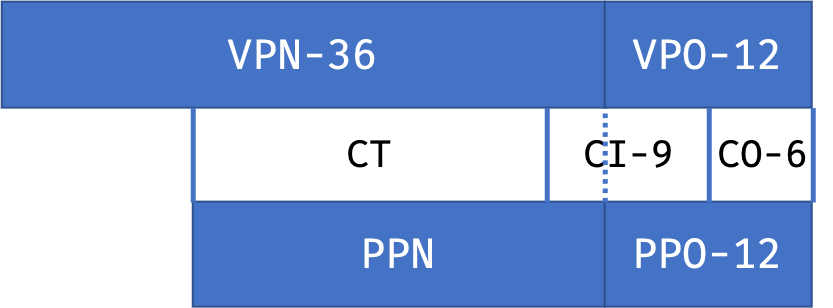
\includegraphics[width=0.5\textwidth]{imgs/1a.png}}
  \caption{Demonstration of bits layout in the Core i19 system}
  \label{fig:1a}
\end{figure}

It is important to recognise that the TLB translation of VPN \textrightarrow{} PPN happens \textbf{at the same time} as the L1 cache figures out which set this line belongs with CI. After the TLB translation, L1 cache would have already targeted the cache set to look into and compare the tag with each cache line thereafter.

In the case of having two processing having the same virtual address to two different physical addresses, it would result in a potential problem named cache homonym. 

\paragraph*{Cache Homonym Example}

Consider two processes that maps virtual address VPN:VPO to PPN1:PPO and PPN2:PPO respectively, the L1 cache would take \textbf{the last 3 bits of VPN and the first 6 bits of VPO} for the set lookup, which would be identical for both processes.

Now that the TLB translates VPN \textrightarrow{} PPN, we are looking at the same cache set in the L1 Cache. Consider a case where the physical address only differs in \textbf {the last 3 bits of PPN1 and PPN2}, we would notice that the Cache Tag is also identical! This creates a problem here as we are looking at two different physical address that maps to the same cache line. The issue lies in the fact that the cache tag itself here would be insufficient to uniquely identify the address.

\subsubsection{}

The Linux kernel is a preemptive multitasking kernel (contrary to uni-kernel). Since each process have their own mapping in their page table, it is very possible that they could map the same virtual address to different physical pages. 

For example, at the text section, two different process would map the same virtual address ($\mathtt{0x400000}$) to their own code respectively, which would very likely be in different physical addresses. 

Another example would be an address in the middle of the virtual memory space that belongs to the heap of each processes (note that it is not the same heap, just the same virtual address). Each process can arbitrary map the allocated heap virtual address to anything it needs during the execution process. So, again, it is very likely to map the same virtual address to different physical addresses.

\subsection{}

\subsubsection{}

With reference to the analysis in section \ref{section:1ai}, we illustrates the issue cache synonym that happens when two processes map the same physical address to two different virtual addresses.

\paragraph*{Cache Synonym Example}

Consider two processes that maps VPN1:VPO and VPN2:VPO both to PPN:PPO. Note that the VPO must match with PPO, due to the address translation process only happens at the top bits of the address. When the L1 Cache is determing which set to look for, again, it would take \textbf{the last 3 bits of VPN1/VPN2 and the first 6 bits of VPO}. Consider a case where the VPN1 differs to VPN2 in the last three digits, the L1 Cache would be looking at two completely different sets given the different Cache Set Index.

Moving on, after the address translation, we would have the same PPN; the L1 Cache would have the same tag, but in different sets. We observe that the same physical address is now mapped to the same tag but different sets in the L1 Cache! Same data getting cached in several different sets (and different lines due to set difference) would yield unexpected results. Consider a write-back cache where the two copies are modified simultaneously, both processes would not see each other's modifications due to different sets/lines. Moreover, the cache would not be able to determine what to write when finally writing down the two (or more) cache lines that belongs to the same physical address to the lower level.

\subsubsection{}

Even for a single process, we can also map the same physical address to multiple virtual addresses. It would also be possible for multiple processes.

For example, \texttt{glibc}'s code, as used by multiple processes, can retain one copy in the physical memory, while being mapped to different virtual addresses of various processes as needed. This is a standard behaviour of the Linux kernel to save memory resources.


\subsection{}

To avoid the aforementioned issues, we need to design a VIPT cache. The key to do so is to make sure the untranslated bits (VPO/PPO) of the address fits in both Cache Set Index and Cache Block Offset. 

Let $s$ be the bit width of set ($S = 2^s$ sets), $e$ be the bit width of lines per set ($E = 2^e$ lines), and $b$ be the bit width of bytes per line ($B = 2^b$ bytes).

Given the virtual page size of $P$ bytes, let $2^p = P$, the VPO shall be $p$-bit wide. Thus $s + b \leq p$. The cache capacity shall be $S \times E \times B$, where $S \times B \leq P$.

Now the greatest L1 data cache capacity is dependent on the associativity of the cache. Thus, we conclude, on a $E$-way set associative cache, for it to be VIPT,
$$ C_{greatest} = P \times E$$

\newpage
\section{}

\subsection{}
First, her implementation would be erroneous when \texttt{strcmp()} encounters a 0, which could mean both the null terminator \texttt{\\0} and the data symbol $\mathtt{0b00}$. Thus, her comparison of two longer strings would most likely terminate early when any of them has a $\mathtt{0b00}$ symbol in the middle.

Second, her implementation would go out of memory bounds when \texttt{strcat()} two strings. As specified in the problem, she only allocates two bytes of memory for a new C string. When she concatenate the two strings together, \texttt{strcat()} would not check for memory boundary, nor would it allocate new memory at the end of the destination string. Most likely, when she accumulated a long enough string, it would write to an invalid page and returns a segfault.

\subsection{}

\subsubsection{}

For implementation 1, it consumes 1 byte for each symbol. It also needs one more byte for the $\mathtt{0xff}$ terminator. Hence, the string itself consumes $n + 1$ bytes. However, to be comparable, we would need a pointer that points to the \texttt{malloc}'d string buffer, which would be 8 bytes on a x86-64 system. In total, this implementation consumes $n + 1 + 8 = n + 9$ bytes.

For implementation 2, it consumes 8 bytes for \texttt{char *s;}, and 2 bytes for \texttt{unsigned short len;}, but another 6 bytes for the 8-byte alignment requirement. Thus, the \texttt{struct symstring} would consume $8 + 2 + 6 = 16$ bytes. The n symbol string now would not need a terminator anymore, as the length is encoded in the struct. In total, that would be $n + 16$ bytes.

Implementation 1 is more memory efficient. Compared to implementation 2, where it uses the extra memory overhead \texttt{struct} to store the string length (with extra alignment), implementation 1 only needs one more \texttt{char 0xff} to act as the terminator.

\subsubsection{}

Implementation 2 is more CPU-efficient when appending newly read input symbol to the end. 

For implementation 1, since we only have the pointer to the start of the section provided by \texttt{malloc}, we would need $O(n)$ (n being the string length) time to traverse the string and find the terminator. Then, we can make changes to the terminator and append strings thereafter.

For implementation 2, we already have the length in the \texttt{struct}. We can essentially "fly" to end and append at \texttt{char* nextsym = s + len}. This is constant time operation with $O(1)$ time. Thus, it shall be more CPU-efficient.

Note that when appending new symbols, we shall be wary of the total allocated memory size and make sure to \texttt{realloc} when necessary.

\subsubsection{}

In implementation 1, we \texttt{malloc} string blocks in table as we go along encoding the file. Since, the LZW encoder never deallocate an individual symbol once it has been added, we can instead \texttt{malloc} reasonably large block of memory at the beginning. As we go along and grew the table, we can \texttt{realloc} the block if needed.

This alternative approach saves both memory and CPU time. Memory wise, we have lower dynamic allocation overhead. CPU wise, besides saving the each \texttt{malloc} calls, we can quickly iterate over the table, as the data in the same block exhibits better spatial locality. Moreover, \texttt{realloc} would reasonably try to expand the block if possible. Only in the case where the block is not expandable, it would then really find another larger block and move our memory there. 

\subsection{}

This second bullet point is incorrect. She should \textbf{increment the \texttt{currwidth} on adding a longer-bit entry to the table}. It can be too late to increment \texttt{currwidth} when the encoder needs to output longer bits of code.

\paragraph*{Error Example}

Let the symbols be 0, 1, 2, 3.

We construct a symbol string: \texttt{0 1 2 3 0 2 1 3}

At the beginning, we should have
\begin{itemize}[topsep=0pt]\itemsep-0.6em 
    \item 0 \textrightarrow{}000
    \item 1 \textrightarrow{}001
    \item 2 \textrightarrow{}010
    \item 3 \textrightarrow{}011
\end{itemize}

We use "|" to show the encoder/decoder progress below.

\textbf{Encoder Stage:} \texttt{0 | 1 2 3 0 2 1 3}
\newline Output: \texttt{000}
\newline New Table Entry: N/A

\textbf{Encoder Stage:} \texttt{0 1 | 2 3 0 2 1 3}
\newline Output: \texttt{000 001}
\newline New Table Entry: 0 1 \textrightarrow{} 100

\textbf{Encoder Stage:} \texttt{0 1 2 | 3 0 2 1 3}
\newline Output: \texttt{000 001 010}
\newline New Table Entry: 1 2 \textrightarrow{} 101

\textbf{Encoder Stage:} \texttt{0 1 2 3 | 0 2 1 3}
\newline Output: \texttt{000 001 010 011}
\newline New Table Entry: 2 3 \textrightarrow{} 110

\textbf{Encoder Stage:} \texttt{0 1 2 3 0 | 2 1 3}
\newline Output: \texttt{000 001 010 011 000}
\newline New Table Entry: 3 0 \textrightarrow{} 111

\textbf{Encoder Stage:} \texttt{0 1 2 3 0 2 | 1 3}
\newline Output: \texttt{000 001 010 011 000 {\color{blue}0010} }
\newline Wrong: \ \texttt{000 001 010 011 000 {\color{red}010} } (no input longer than 3 bits detected)
\newline New Table Entry: 0 2 \textrightarrow{1000}

\textbf{Encoder Stage:} \texttt{0 1 2 3 0 2 1 | 3}
\newline Output: \texttt{000 001 010 011 000 0010 {\color{blue}0001} }
\newline Wrong: \ \texttt{000 001 010 011 000 010 {\ \color{red}001} } (similar as above)
\newline New Table Entry: 2 1 \textrightarrow{1001}

\textbf{Encoder Stage:} \texttt{0 1 2 3 0 2 1 3 |}
\newline Output: \texttt{000 001 010 011 000 0010 0001 {\color{blue}0011} }
\newline Wrong: \ \texttt{000 001 010 011 000 010 001  {\ \ \color{red}011} } (similar as above)
\newline New Table Entry: 1 3 \textrightarrow{1010}

With the error-nous encoder, we now have the compressed string :

\texttt{\color{red}000 001 010 011 000 010 001 011}

The correct compressed string shall be:

\texttt{\color{blue}000 001 010 011 000 0010 0001 0011}

We initialise the table entry as below and start decoding
\begin{itemize}[topsep=0pt]\itemsep-0.6em 
    \item 0 \textrightarrow{}000
    \item 1 \textrightarrow{}001
    \item 2 \textrightarrow{}010
    \item 3 \textrightarrow{}011
\end{itemize}

\textbf{Decoder Stage:} \texttt{000 | 001 010 011 000 010 001 011}
\newline Output: \texttt{0}
\newline New Table Entry: N/A

\textbf{Decoder Stage:} \texttt{000 001 | 010 011 000 010 001 011}
\newline Output: \texttt{0 1}
\newline New Table Entry: 0 1 \textrightarrow{} 100

\textbf{Decoder Stage:} \texttt{000 001 010 | 011 000 010 001 011}
\newline Output: \texttt{0 1 2}
\newline New Table Entry: 1 2 \textrightarrow{} 101

\textbf{Decoder Stage:} \texttt{000 001 010 011 | 000 010 001 011}
\newline Output: \texttt{0 1 2 3}
\newline New Table Entry: 2 3 \textrightarrow{} 110

\textbf{Decoder Stage:} \texttt{000 001 010 011 000 | 010 001 011}
\newline Output: \texttt{0 1 2 3 0}
\newline New Table Entry: 3 0 \textrightarrow{} 111

{\color{red} last entry in 3 bits, time to increment bit width and expect 4 bit symbols now}

\textbf{Decoder Stage:} \texttt{000 001 010 011 000 {\color{red}(010 0)} | 01 011}
\newline Output: \texttt{0 1 2 3 0 {\color{red}0 1}}
\newline New Table Entry: 0 0 \textrightarrow{} 1000

\textbf{Decoder Stage:} \texttt{000 001 010 011 000 (010 0) {\color{red}(01 01)} | 1}
\newline Output: \texttt{0 1 2 3 0 0 1 {\color{red}1 2}}
\newline New Table Entry: 0 1 1 \textrightarrow{} 1001

\textbf{Decoder Stage:} \texttt{000 001 010 011 000 (010 0) (01 01) {\color{red}1}}
\newline Output: \texttt{0 1 2 3 0 0 1 1 2}
\newline \texttt{Invalid decoder input: aborting}, why is there only 1 bit left?

Hence, the decoder outputs an error, with the output string \texttt{0 1 2 3 0 0 1 1 2} different from \texttt{0 1 2 3 0 2 1 3}.

In conclusion, we showed that the encoder should have increased the \texttt{currwidth} on adding the first longer-bit table entry.


\newpage
\section{}

\newpage
\section{}

\subsection{}

\subsubsection{}

As described above, we consider \texttt{malloc()/free()} a function that does the following:
\begin{itemize}[topsep=0pt]\itemsep-0.6em 
    \item \texttt{spinlock.lock();}
    \item \texttt{// operates on the heap}
    \item \texttt{spinlock.unlock();}
\end{itemize}

Consider the parent process's two threads, $T_1$ is in the middle of a \texttt{malloc()}, while $T_2$ is \texttt{fork()}-ing a child process. Note that the lock is now in the hands of $T_1$'s \texttt{malloc()}. 

As described above, calling \texttt{fork()} on a multi-threaded program would \textbf{only fork the single thread that actually called it}. However, \textbf{the entire virtual address space of the parent process is replicated in the child}, including the states of spinlocks. In other words, only $T_{2forked}$ exists, while $T_{1forked}$ is not there anymore to unlock its locked $\mathtt{spinlock}_{forked}$. Thus, when $T_{2forked}$ invokes \texttt{malloc()} later on in the logic flow, the locked $\mathtt{spinlock}_{forked}$ (but never can be unlocked) would result in a deadlock and hangs the child process.

\subsubsection{}

No, she is not correct.

Being async-signal-safe a function means that the function is either reentrant, or uninterruptible by signals (uninterruptible system calls). If a function is reentrant, it can be interrupted in the middle of an execution and safely called again, before completing its previous invocation. \texttt{malloc()} would clearly would not be able to achieve this as it operates on a globally shared data structure.

Consider a single-threaded process where \texttt{malloc()} is invoked normally, and in its signal handlers. Signals can arrive at anytime of execution, hence asynchronous. In the case where a signal arrives during the \texttt{malloc()} process in the logic flow, the signal handler would be invoked. 

If it is a thread-safe \texttt{malloc()}, the logic flow \texttt{malloc()} would be holding the heap lock, waiting for the signal handler to finish. The signal hanlder, on the other hand, is waiting for its \texttt{malloc()} to acquire the heap lock. This results in a unfortunate deadlock situation.

Now we consider removing the locks of the \texttt{malloc()} (or if we use a reentrant lock in C++). Then, the signal handler's \texttt{malloc()} (in the same thread as the logic flow) would encounter a half-modified heap state, and could potentially corrupt the heap structure by allocating new blocks on top of it.

In all, as we have shown, \texttt{malloc()} is \textbf{not async-signal-safe}, with or without the process-wide spinlock on the heap.

\subsection{}

\subsubsection{}

The string \texttt{"Hello"} is printed twice due to the output is line-buffered in C's Standard I/O.

When the first \texttt{printf("Hello")} is called, the string \texttt{"Hello"} is put into the buffer for \texttt{stdout}. Since the \texttt{stdout} is line-buffered by default, we would not see the string on the screen yet.

Then the \texttt{fork()} happens. As mentioned previously, \texttt{fork()} copies the entire virtual address space to the child in a copy-on-write fashion, including the \texttt{stdout} buffer. Now, we have two copies of the \texttt{stdout} buffer, both with the string \texttt{"Hello"}.

The child process than calls \texttt{printf("Child goodbye\textbackslash n")} with a newline. Since there is a newline, the whole string in the child's buffer \texttt{"HelloChild goodbye"} would be presented on the console. The same happens for the parent process as well (\texttt{"HelloParent goodbye"}). Therefore, there are two \texttt{"Hello"}s in total.

\subsubsection{}

Here we offer two ways to force the output \texttt{"Hello"} to be generated once.

First, we can simply turn off the buffer on the \texttt{stdout} stream as shown in the code listing \ref{lst:4bii-nobufstdio} above. Thus everything printed using Standard I/O to \texttt{stdout} will be turned into a \texttt{write()} system call immediately. 

\begin{lstlisting}[style=C++, label={lst:4bii-nobufstdio}, caption={Turn off buffer for \texttt{stdout}},captionpos=b]
#include <stdio.h>
#include <unistd.h>

int main () {
  (*@\textbf{setvbuf(stdout, NULL, \_IONBF, 0);}@*)
  printf("Hello");
  if (fork() == 0) {
    printf("Child goodbye\n");
  } else {
    printf("Parent goodbye\n");
  }
  return 0;
}
\end{lstlisting}

The other way would be to flush the \texttt{stdout} buffer before \texttt{fork()}, as shown in listing \ref{lst:4bii-flush}.

\begin{lstlisting}[style=C++, label={lst:4bii-flush}, caption={Flush the \texttt{stdout} buffer before \texttt{fork}},captionpos=b]
#include <stdio.h>
#include <unistd.h>

int main () {
  printf("Hello");
  (*@\textbf{fflush(stdout);}@*)
  if (fork() == 0) {
    printf("Child goodbye\n");
  } else {
    printf("Parent goodbye\n");
  }
  return 0;
}
\end{lstlisting}


\newpage
\section{}




\end{document}